\documentclass[informe.tex]{subfiles}
\begin{document}
Este tipo de filtro consiste en relacionar las especificaciones de retardo de fase lineal o de grupo constante del filtro ideal con los polinomios de la función de transferencia.\newline

El retardo de grupo es de particular importancia cuando es relevante las formas de onda de la señal. Por ejemplo para señales de audio, no es perceptible los cambio de fase, pero para señales de vídeo es importante conservar la forma de onda.  Las funciones obtenidas de esta manera tienen un \underline{retraso plano máximo en el origen}.\\

La función de Bessel aproxima a una constante de retardo de un filtro pasa bajo.\\  

\textbf{Función de aproximación:}\\\\

El polinomio de Bessel definido en forma cerrada es:
		$$	
		B_n(\tau_0 s )=s^n + b_{n-1} s^{n-1} + ... + b_1 s + b_0
		$$
donde es $b_k = \frac{(2n - k)!}{2^{n-k} k! (n-k)!}$ y n es el orden del polinomio.\\

Por otro lado, la forma recursiva esta dada por:
	$$
	B_n(s) =
	\left \{ 
	    \begin{matrix}
		1                             		& \mbox{, para } n=0\\
     	s+1                           		& \mbox{, para } n=1\\
   		(2n-1) B_{n-1}(s)- s^2 B_{n-2}(s) & \mbox{, otro valor}
	    \end{matrix}
	\right.		
	$$    
		
	\textbf{Función de transferencia}

		\[	
			H(s) = \frac{K}{e^{\tau_0 s}} = \frac{K}{s^n + b_{n-1}s^{n-1} + ... + b_1 s + b_0}
		\]
	
 	donde $K$ se elige tal que $H(0)=1$ y por lo tanto $K=b_0$;  $\tau_0$ es la constante de fase y los coeficientes del polinomio se pueden obtener de dos formas:\newline
 	1- Igualación de parámetros, o\newline
 	2- Desarrollo de polinomios de Bessel.\newline
 	
\textbf{1- Método por igualación de parámetros}\newline

Planteando la función de transferencia en $s$ tal como: 	
		
	$$
		H(s)= 
 			\frac{K}{e^{\tau_0 s}} 
		    =
		      \frac{K}{cosh(s)+sinh(s)}
		    =
		      \frac{K}{s^n + b_{n-1}s^{n-1} + ... + b_1 s + b_0}
		    = 
		      \frac{K}{M(s)+N(s)}
 			= K \left( 
		     		\frac{M(s)-N(s)}{M^2(s)-N^2(s)}
		     	\right)		   		     
	$$
donde el par transformado de $H(s)$ viene dado por
	$$
		h(t) = K \delta(t - \tau_0) 
            \xleftrightarrow[]{\mathscr{L}}
		H(s) = K e^{-\tau_0 t}
	$$
así $H(s)$ se relaciona con la función de transferencia a partir de los polinomios en s, siendo $s=j \omega$, la fase queda definida por
   \begin{equation}
		\label{eqn:bessel:fase:1} 
		\varphi(\omega)= - atanh \left(\frac{N(\omega)/j}{M(\omega))} \right)
			               = - atan \left(
			                            \frac{b_1 \omega}{ -\omega^2 + b_0}
			                       \right)
	\end{equation}
	
El retardo de grupo,  $\tau(\omega)$,  es la derivada de la fase $\varphi(\omega)$
		$$
			\tau(\omega) \triangleq -\frac{ d \varphi (\omega)}
			               { d \omega}
			        = - \frac{u'}{1+u^2} =T   \mbox{ siendo } u=\frac{N(\omega)/j} {M(\omega)} \mbox{ y } T \mbox{ es una constante.}
		$$
desarrollando lo anterior para una retardo de grupo normalizado, con $T=1$,
   \begin{equation}
		\label{eqn:bessel:retardo_grupo:1} 
		\tau(\omega) = - \frac{ -atan \left( 
		                      -\frac{b_1 \omega}{-\omega^2 +b_0}
		                              \right)}
		                     { d\omega}
		             = \frac{b_1 \omega^2 + b_1 b_0}
                    {\omega^4 + (-2 b_0 + b_1^ 2)\omega^2 + b_0^2}
                    = 1
	\end{equation}
Entonces, la máxima planicidad de retardo de grupo implica que $\tau(0)=1$, de la Ec. \ref{eqn:bessel:retardo_grupo:1} se despeja 
	\begin{equation}
		\label{eqn:bessel:retardo_grupo:b1} 
		\frac{b_1 \cancel{b_0}}{b_0^{\cancel{2}}}=1 \longrightarrow b_1=b_0
	\end{equation}

Operando la Ec. \ref{eqn:bessel:retardo_grupo:1}	
	$$
		b_1 \omega_1^2 + b_1 b_0 = \omega^4 + (-2 b_0 + b_1^2) \omega^2 + b_0^2
	$$	
y de esta ultima expresión reemplazando con lo obtenido en la Ec. \ref{eqn:bessel:retardo_grupo:b1} se tiene 
	$$
		\omega^4 + (-3 b_0 + b_0^2) \omega^2 = 0
	$$
el segundo término debe ser cero, entonces
	\begin{equation}
		\label{eqn:bessel:retardo_grupo:b0} 
		(-3 \cancel{b_0} + b_0^{\cancel{2}})=0 \longrightarrow b_0=3
	\end{equation}
por lo tanto, $b_1=3$, la función de transferencia es
	\begin{equation}
		\label{eqn:bessel:retardo_grupo:b0} 
		H(s)=\frac{b_3}{s^3 + 3 s + 3}
	\end{equation}	
	
\textbf{2- Desarrollo en polinomios de Bessel}\\	

Partiendo de que $$ H(s)= \frac{K}{ e^{\tau_0 s}} = \frac{K}{ cosh(s)+sinh(s)}$$  la fase se podría plantear mediante el cociente de $cosh(s)$ y de $sinh(s)$, y luego con los desarrollos de serie de Taylor se puede llegar a 
	\begin{equation}
		\label{eqn:bessel:polinomio} 
\varphi_2(s) =\frac{cosh(s)}{sinh(s)}
		            =\frac{1 - \frac{s^2}{2!} +  \frac{s^4}{4!} -  \frac{s^6}{6!}+ ...}
		                  {1 - \frac{s^3}{3!} +  \frac{s^5}{5!} -  \frac{s^7}{7!}+ ...}
		            =\frac{1}{s} + \frac{1}{\frac{3}{s} + \frac{1}{\frac{5}{s}+ \frac{1}{\frac{7}{s} + ...}}}				                  
	\end{equation}

el desarrollo de la división continuada queda como sigue:
	\begin{center}
		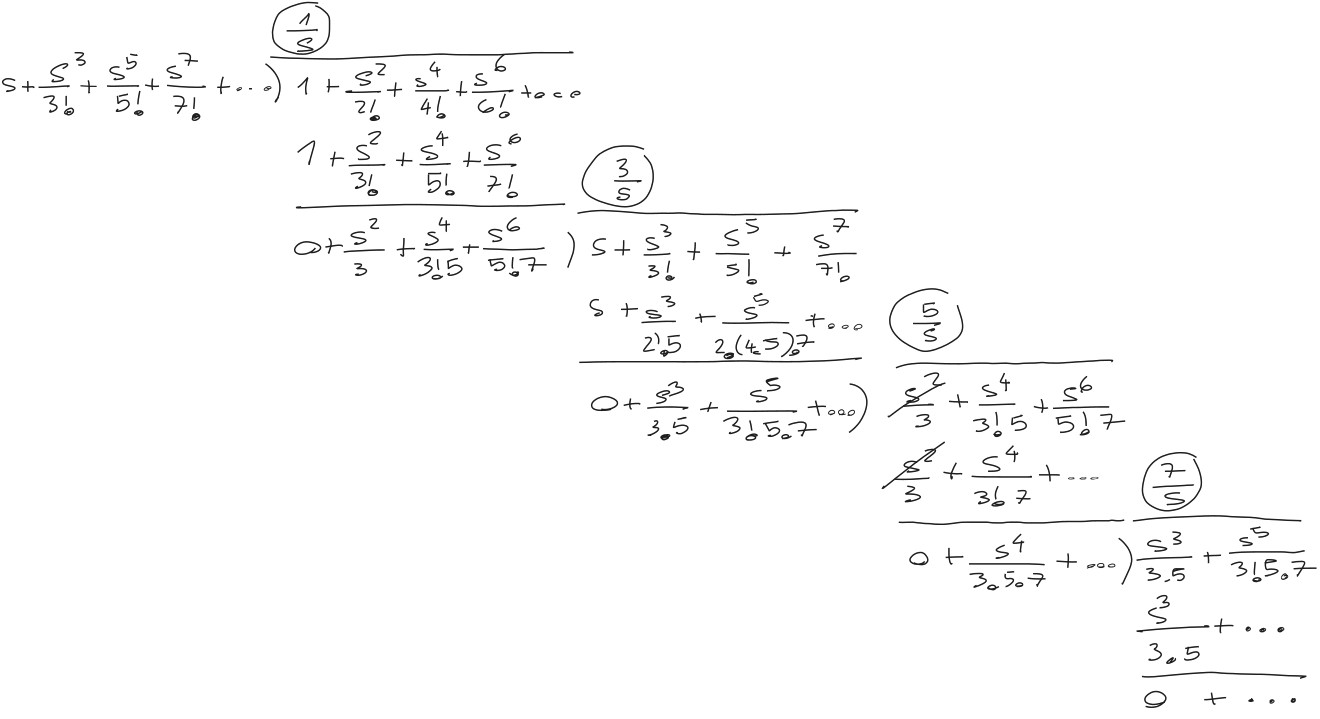
\includegraphics[scale=1]{bessel_3.jpg}
	\end{center}		
	
Para el caso de un orden 2, de la Ec. \ref{eqn:bessel:polinomio} se puede asociar el numerador de la fase a la parte par del denominador del polinomio de la función de transferencia, y de igual forma para con el denominador de la fase, quedando que 
	$$
		\varphi_2(s) = \frac{1}{s} + \frac{1}{\frac{1}{s}} = \frac{3+s^2}{3s} = \frac{M(s)}{N(s)}
	$$
Entonces la función de transferencia queda como;
	\begin{center}
		$H(s)=\frac{K}{M(s)+N(s)}=\frac{K}{1+s^2+3s}$ donde $k=3 \mbox{ para que } H(0)=1$ 	
	\end{center}

%%		
\textbf{\newpage Ejemplo con Matlab 1:} Filtro pasa bajo de Bessel, Fig. \ref{fig:func:bessel:ej1}. \newline 
  
\lstinputlisting[language=Matlab, frame=single]{./src_matlab/bessel_ej1.m}     
    	
\begin{figure}[h]
     \centering
     \begin{subfigure}[b]{1\textwidth}
         \centering
         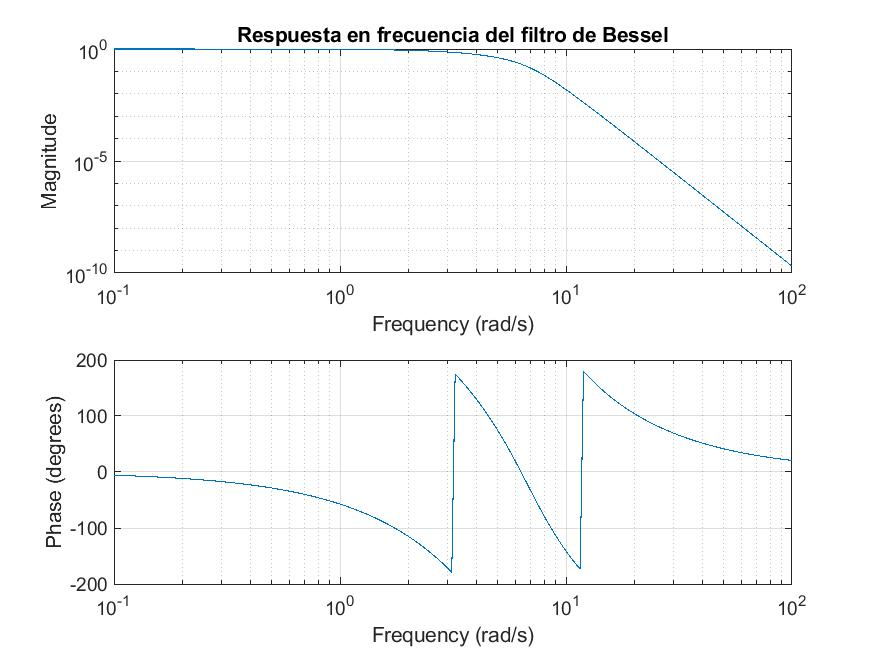
\includegraphics[scale=0.35]{bessel_ej1_freqs.jpg}
         \caption{Respuesta en frecuencia del filtro Bessel del Ejemplo 1}
         \label{fig:func:bessel:ej1:freqs_bp}
     \end{subfigure}
\end{figure}     

\begin{figure}[h]
	\ContinuedFloat
     \begin{subfigure}[b]{1\textwidth}
         \centering
         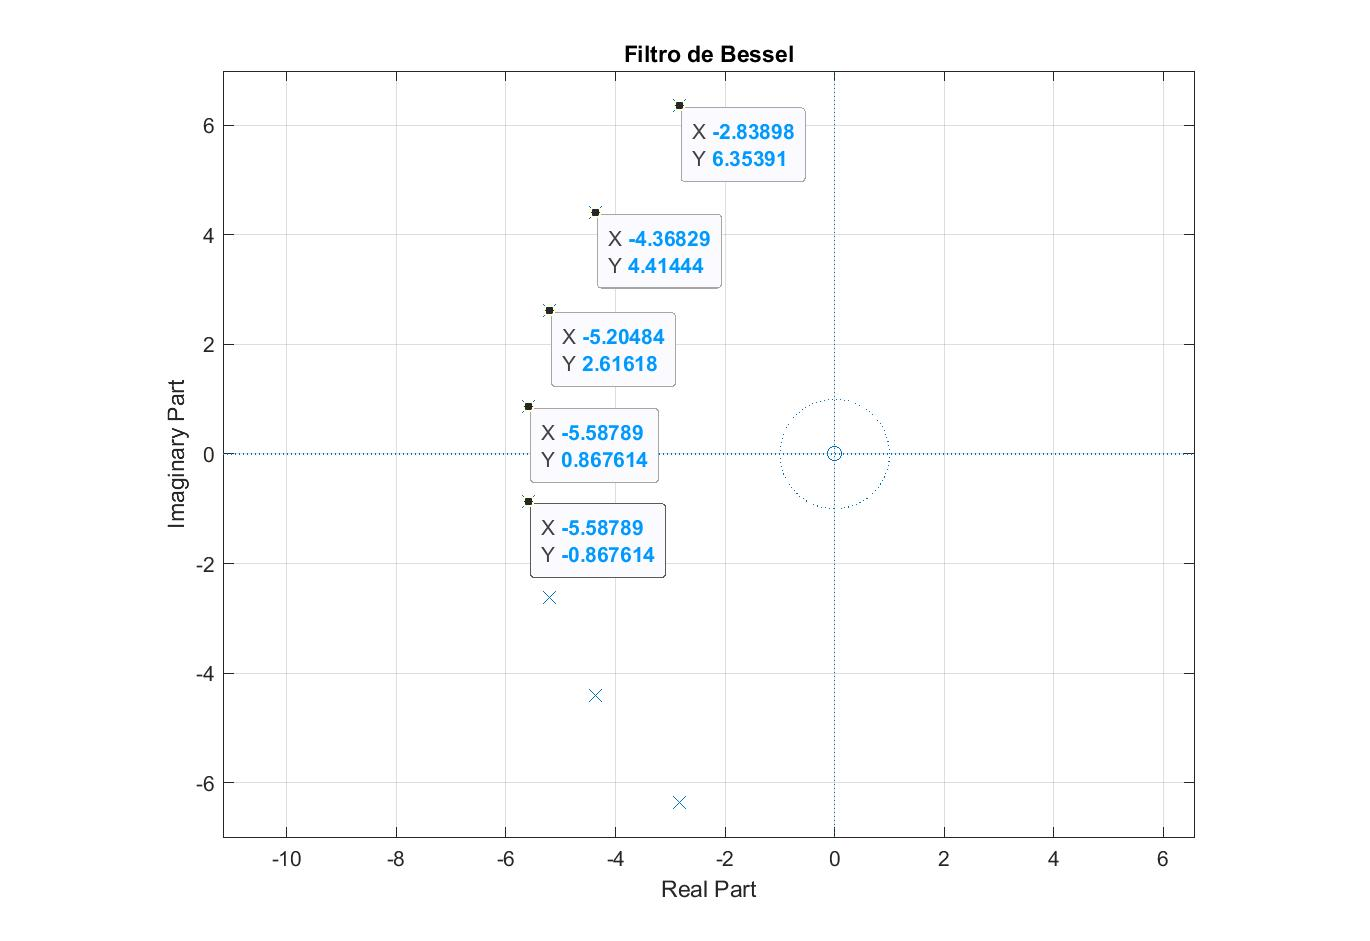
\includegraphics[scale=0.35]{bessel_ej1_pz.jpg}
         \caption{Diagrama de polos y ceros del filtro de Bessel del Ejemplo 1}
         \label{fig:func:bessel:ej1:pz}
     \end{subfigure}
     \caption{Ejemplo 1. Filtro pasa bajo de Bessel}
     \label{fig:func:bessel:ej1}
\end{figure}
 
\end{document}
